\section{PDCA}\label{PDCASection}
Il PDCA è un modello studiato per il miglioramento continuo della qualità di un prodotto a lungo raggio. Fondamento di questo metodo è promuovere un tipo di cultura orientata al miglioramento continuo dei processi e all'utilizzo ottimale delle risorse. Il nome di fatto è un acronimo qui scomposto:
\begin{center}
	\item \textbf{P}lan-\textbf{D}o-\textbf{C}heck-\textbf{A}ct
\end{center}
Difatti questo metodo è scomposto in quattro fasi qui descritte:
\begin{itemize}
	\item \textbf{Plan}: consiste nella definizione di ciò che bisogna essere fatto per affrontare e risolvere un problema o migliorare un processo;
	\item \textbf{Do}: in questa fase vengono attuate le soluzioni ed i piani precedentemente definiti, eseguendo il programma;
	\item \textbf{Check}: test e controllo, si studiano i risultati ottenuti dall'esecuzione del programma (rilevati nel "DO") confrontandoli con i risultati attesi (trovati nel "PLAN"); 
	\item \textbf{Act}: è la fase finale di applicazione definitiva delle migliorie trovate e definite nei processi precedenti; si individuano altre opportunità di miglioramento che richiederanno altri cicli per apportare le dovute modifiche.
\end{itemize}
In sostanza il PDCA è un modello che fissati gli obiettivi iniziali e soddisfatti, si passa a fissare nuovi obiettivi da raggiungere per alzare il livello della qualità.

\begin{figure}[H]
\centering
	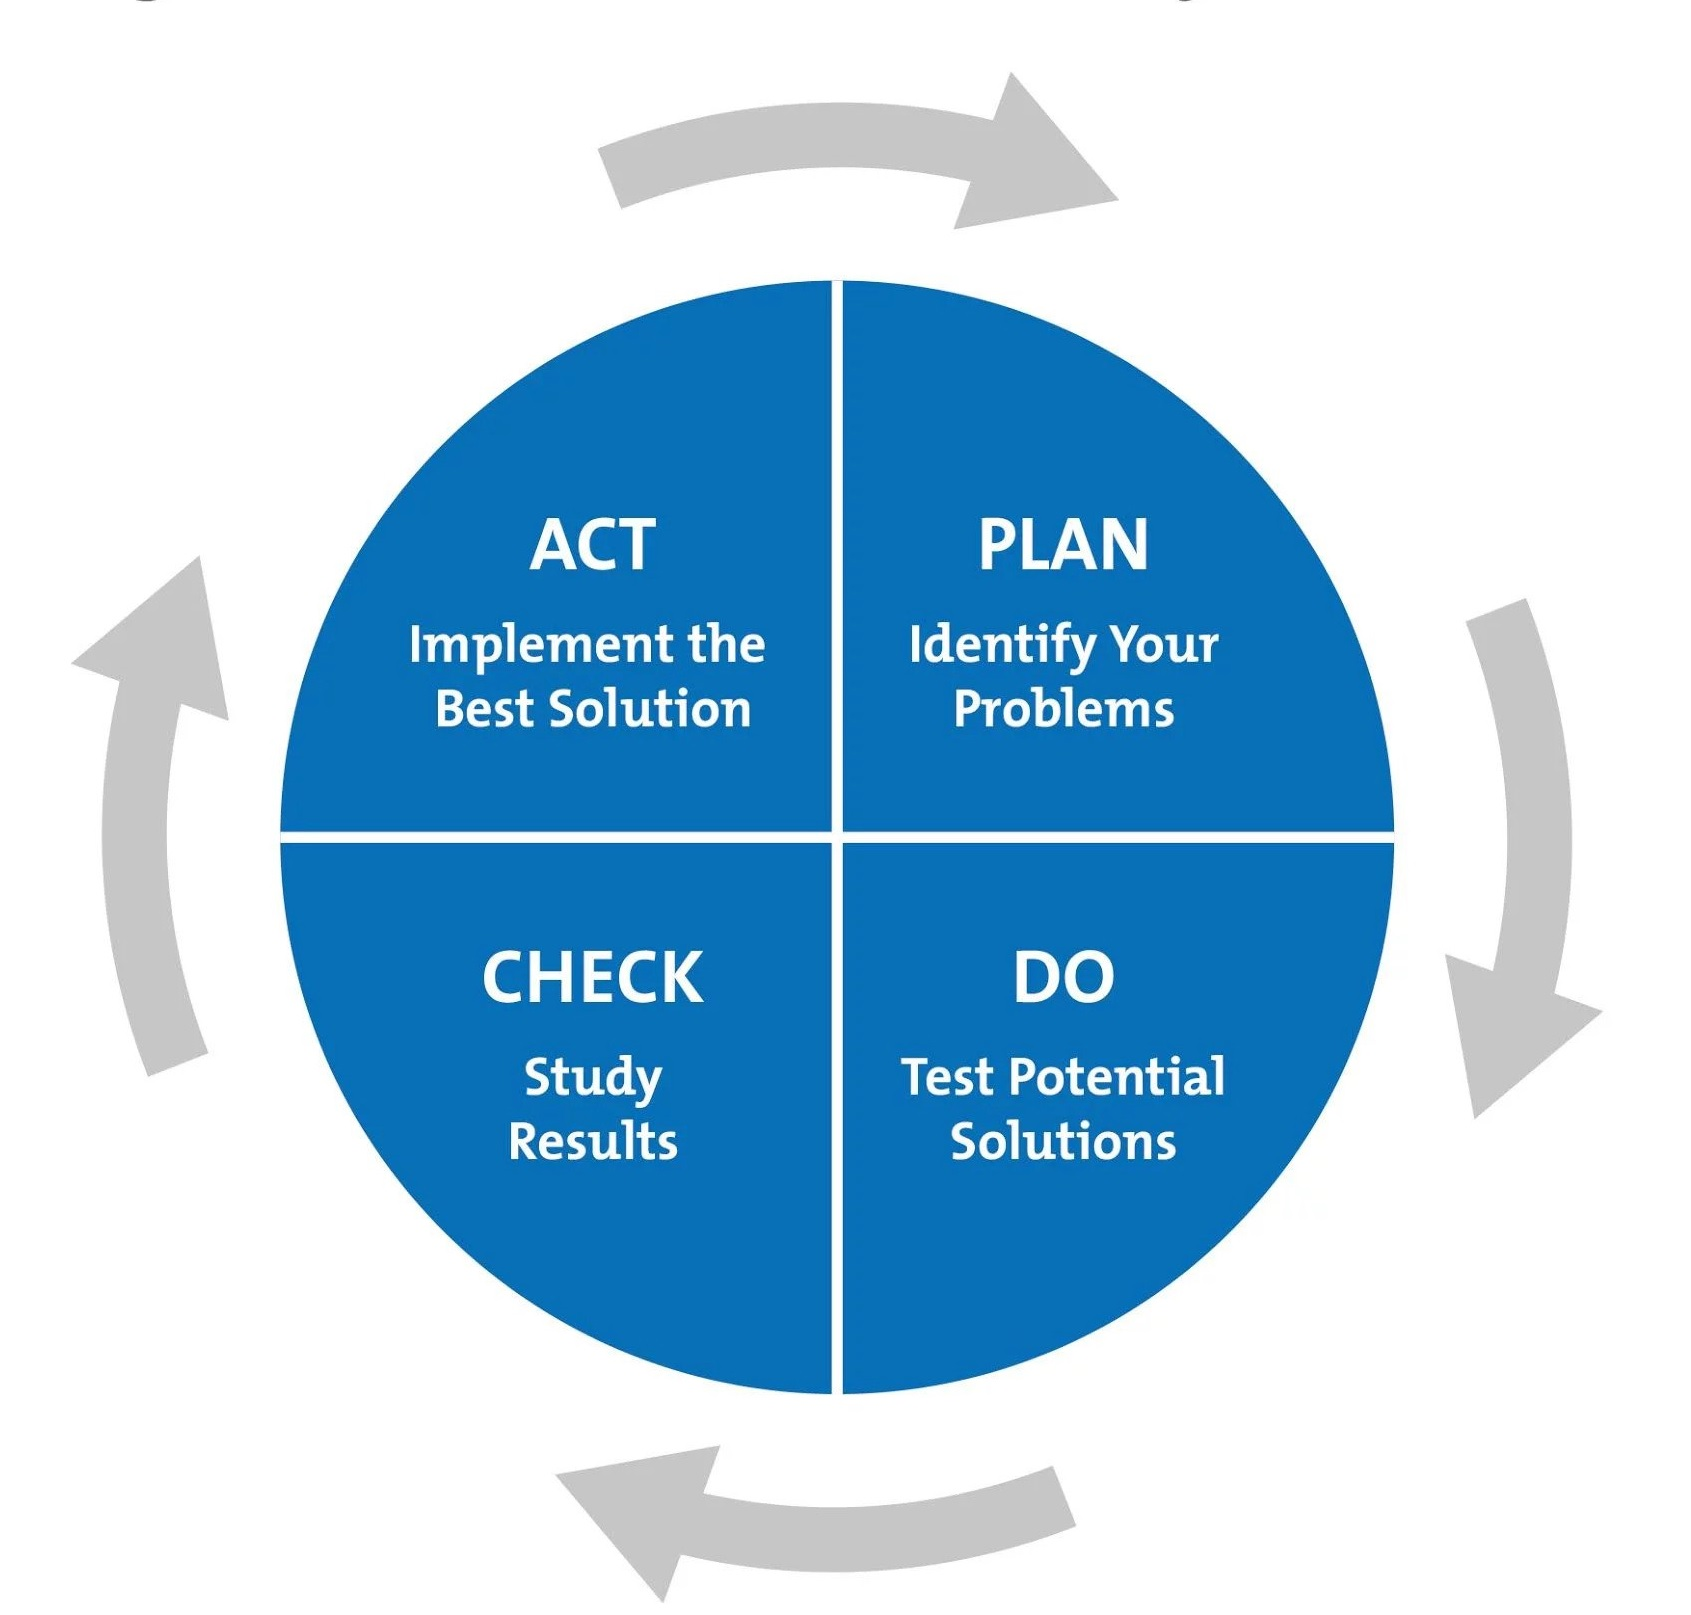
\includegraphics[width=0.4\linewidth]{./images/pdca.jpg}
	\caption{Modello PDCA}
	\label{pdca}
\end{figure} 

 